\documentclass{examnotes}

\def\disobeylines{\catcode`\^^M=5 }
\header{STA2601 Applied Satistics II}

\begin{document}

\obeylines
\setlength\baselineskip{15pt}
\h{STA2601 Applied Satistics II}
\h{Chapter 1}

{\it Integral} is the distribution function, or cumulative probability function,  $F_X(x)$ \\
{\it Derivative} is the probability function, or probability density function $f_x(x)$

\ml{Z=\frac{X-\mu}{\sigma}}
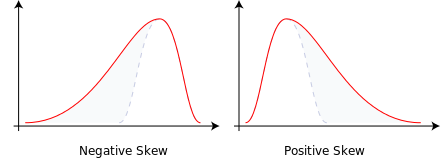
\includegraphics[scale=0.6]{./img/skewness.png}

Exponential distribution: $\displaystyle\frac{1}{k}e^{-\displaystyle\frac{x}{k}}$ parameter is $k$.
\vspace{6pt}
$\mu=\Epsilon(X)=\displaystyle\int_{-\infty}^\infty xf_X(x)\ dx$
\vspace{6pt}
$\sigma^2=\Epsilon(X-\mu)^2=\displaystyle\int_{-\infty}^\infty (x-\mu)^2f_X(x)\ dx$
\vspace{6pt}

$\text{Var}(X+Y) =\text{Var}(X)+\text{Var}(Y)+2\text{Cov}(X,Y).$
\vspace{6pt}


\disobeylines
\mymath{
Cov(X,Y)
&= \operatorname{E}\left[\left(X - \operatorname{E}\left[X\right]\right) \left(Y - \operatorname{E}\left[Y\right]\right)\right] \\
&= \operatorname{E}\left[X Y\right] - \operatorname{E}\left[X\right] \operatorname{E}\left[Y\right].
} %\mymath

\obeylines
\h{Study Unit 2}
\ra Unbiased estimator ${\Epsilon(T)=\theta}$ 
\ra $Var(cX)=c^2Var(X)$
\ra Most efficient estimator has the smallest variance. 

Least squares estimation:      
\rn{1} ${Q(\theta_1,\dots,\theta_k)= \displaystyle\sum_{i=1}^n(X_i-\Epsilon(X_i))^2}$
\vspace{6pt}
\rn{2} Replace $\Epsilon(X_i)$ with given ${\theta}$
\vspace{6pt}
\rn{3} Take partials ${\displaystyle\frac{\partial Q}{\partial \theta_j}}$ 
\vspace{6pt}
\rn{4} Set partials ${=0}$ and solve for each ${\hat{\theta_i}}$ then solve simultaneousness equations.

\vspace{6pt   }
Maximum likelihood estimation: (MLE)
\rn{1} Get likelihood function ${L(\theta)=f_X(X_1,\theta)f_X(X_2,\theta)\dots f_X(X_n,\theta)=\displaystyle\prod_{i=1}^nf_X(X_i,\theta)}$
\vspace{6pt}
\rn{2} Take log of likelihood function if needed 
\vspace{6pt}
\rn{3} Take partials ${\displaystyle\frac{\partial Q}{\partial \theta_j}}$
\vspace{6pt}
\rn{4} Set partials ${=0}$ and solve for ${\hat{\theta}}$ \quad\red{! Remember hat \ ${\hat{}}$}

\vspace{6pt}
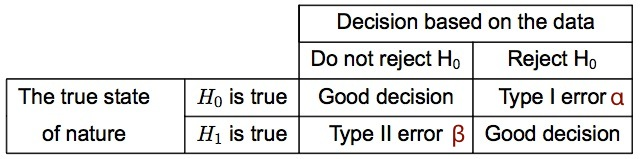
\includegraphics[scale=0.5]{./img/typeerrors.jpg}

Significance level $\alpha = P(H_0 \text{ is rejected}|H_0 \text{ is true})$

Power of the test $ 1-\beta = P( \text{ not rejecting } H_0 | H_1 \text{ is true})$

Confidence level $1-\alpha$

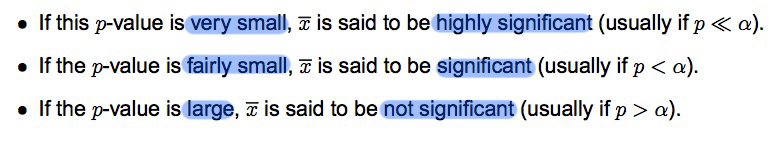
\includegraphics[scale=0.5]{./img/pvalues.jpg}

$\displaystyle\frac{(n-1)S^2}{\sigma^2} \ \mytilde\   \chi^2_{n-1} = \displaystyle\sum_{i=1}^n \left(\frac{X_i-\bar{X}}{\sigma}\right)^2$

$Var(X) = \Epsilon(X_i^2)-[\Epsilon(X_i)]^2$

\vspace{6pt}
$\bar{X} \ \mytilde\ n\left(\theta,\displaystyle\frac{\sigma^2}{n}\right) \quad Z=\displaystyle\frac{\sqrt{n}(\bar{X}-\theta)}{\sigma}$

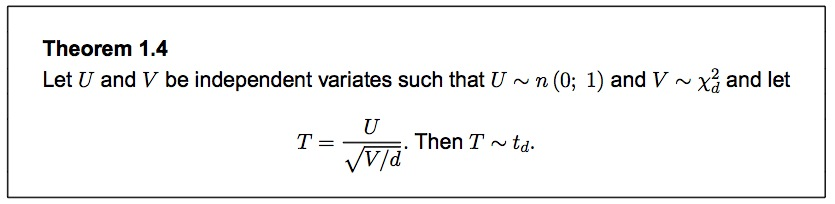
\includegraphics[scale=0.45]{./img/thereom14.jpg}

$\Epsilon(X_i^2)=\theta+\mu^2 \quad \Epsilon(\bar{X}^2)=\frac{\theta}{n}+\mu^2$
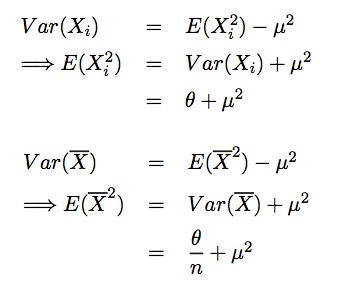
\includegraphics[scale=0.45]{./img/proof1.jpg}

\h{Study Unit 4} 
Van der Waerden's formula: $\displaystyle\frac{r_i}{n+1}$

\sh{$\mathbf{\chi^2}$ Goodness-of-fit test:}
\vspace{6pt}
$Y^2=\displaystyle\sum_{i=1}^k \frac{(N_i - n\pi_i)^2}{n\pi_i}$
$k$ number of intervals
$N_i$ is then number of items falling into the interval calculated from $X_i=\sigma Z+\mu$
$n\pi_i$ is interval weighting X number of observations. 
\vspace{6pt}
\red{\Large If $\mathbf{n\pi_i < 5}$ then pool two or more cells}
\vspace{6pt}
$Y^2 \mytilde \chi^2_{k-1}$ if distribution is fully specified, otherwise 
$Y^2 \mytilde \chi^2_{k-1-r}$ where $r$ is number of unknown parameters.
\vspace{6pt}
Hypotheses:
$H_0$: The sample comes from a $n(\mu,\sigma^2)$ distribution
$H_1$: The sample does not come from a $n(\mu,\sigma^2)$ distribution

Reject null hypothesis if $Y^2>\chi^2_{k-1-r}$

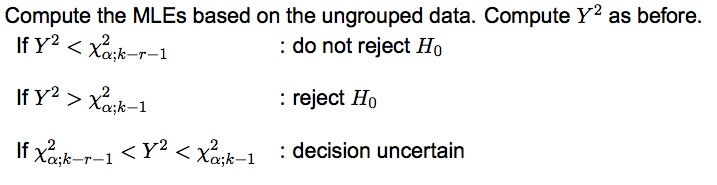
\includegraphics[scale=0.45]{./img/normaltest.jpg}
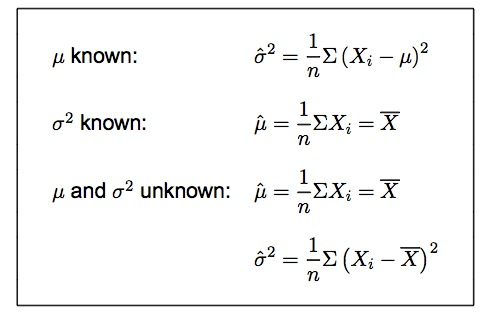
\includegraphics[scale=0.45]{./img/normals.jpg}
Use above when testing grouped data from a normal distribution because MLE's are difficult to compute.

\sh{Method of moments test for normality}
\red{Must perform two hypotheses tests}
{\bf Skewness}
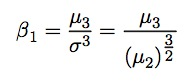
\includegraphics[scale=0.6]{./img/b1.jpg}
Hypotheses:
$H_0$: $B_1=0$ i.e. symmetric
\ra One-sided $H_1$: $B_1<0$ Reject if $B_1 < -TableValue$ or $H_1$: $B_1>0$ Reject if $B_1>  TableValue$. 5\% level
\ra Two-sided $H_1$: $B_1\ne0$ Reject if $|B_1| > TableValue$. 10\% level 
\vspace{6pt}
{\bf Kurtosis} 
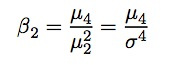
\includegraphics[scale=0.6]{./img/b2.jpg}
Hypotheses:
$H_0$: $B_2=3$ i.e. from normal distribution
$B_2>3$ leptokurtic
$B_2<3$ platykurtic
\vspace{6pt}
\hspace{-5pt}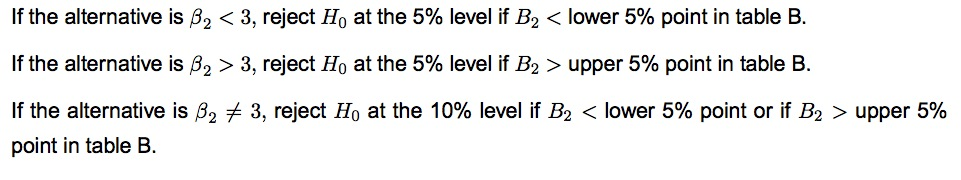
\includegraphics[scale=0.5]{./img/b2tests.jpg}

Use {\bf standardised mean deviation} to test kurtosis if sample size is smaller than 50, statistic $A$
Same hypotheses as $B_2$, 4th moment test.

\vspace{6pt}
$\sum(X_i-\bar{X})^2=\sum X^2_i-n\bar{X}^2$

\h{Study Unit 5}

\sh{Contingency Table Analysis}

Fixed Grand total:
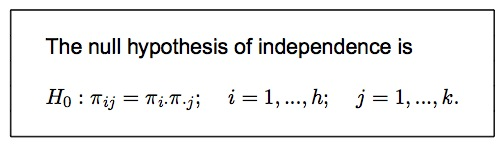
\includegraphics[scale=0.5]{./img/grandtotal.jpg}

Fixed row or column totals:
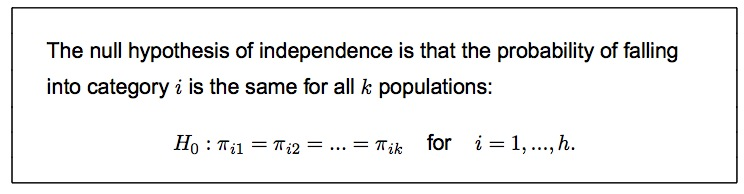
\includegraphics[scale=0.5]{./img/fixedrow.jpg}

Test Statistic:
$e_{ij}=\displaystyle\frac{N_{i.}N_{.j}}{N_{..}}$
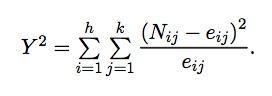
\includegraphics[scale=0.5]{./img/statisitc.jpg}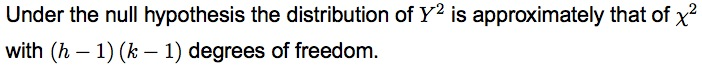
\includegraphics[scale=0.5]{./img/t51.jpg}
Two sided test only i.e. $|Y^2|$.
\vspace{6pt}
\red{\Large Don't forget to pool  $ \color{red}\mathbf{e_{ij} < 5}$ }

\sh{Exact test for 2x2 table}
Discreet Distribution           
Find smallest row/column as $k$ then smallest other as $n$ and $x$ is the cell frequency.

$H0$: There is no association between attribute A and Attribute B
$H1$: Have to figure it out. (Is the value of $x$ unusually to large or small to ascribe to chance.
One sided:
Two sided test $\frac{\alpha}{2}$ reject $H_0$ if $x$ is a rare event.

\sh{Correlation}

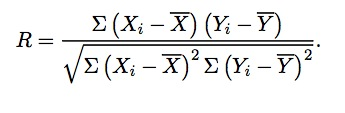
\includegraphics[scale=0.5]{./img/r1.jpg}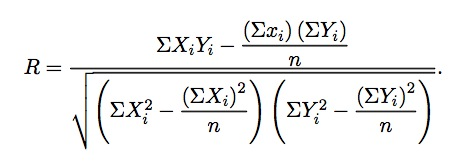
\includegraphics[scale=0.5]{./img/r2.jpg}
In using R $X$ and $Y$ should follow conditions for bivariate normality:
\rn{1} Marginal normality
\rn{2} Linearity

\sh{Testing for zero correlation $\rho=0$}
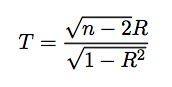
\includegraphics[scale=0.5]{./img/tcor.jpg} 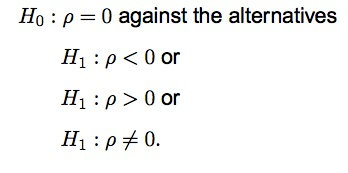
\includegraphics[scale=0.5]{./img/thyp.jpg}
Student's t-distribution $\mytilde\ T_{n-2}$

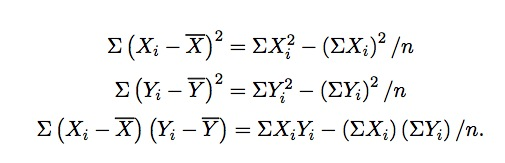
\includegraphics[scale=0.5]{./img/altcov.jpg}
Correlation between X and Y is the same for any linear transformation of X or Y with positive coefficients.

\sh{Fisher's Z-transformation for $\rho\ne0$}
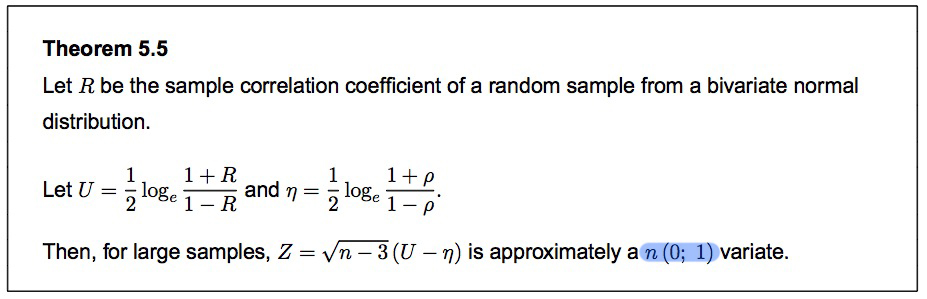
\includegraphics[scale=0.45]{./img/fischer.jpg}
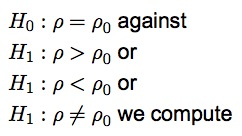
\includegraphics[scale=0.5]{./img/fishhyp.jpg}
 
\sh{Confidence interval for $\mathbf{\rho}$}
Do algebraic transformation on $1-\alpha=P(a<Z<b)$ with $Z=$(fisher transform) and then use 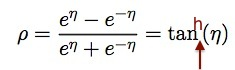
\includegraphics[scale=0.5]{./img/ntrans.jpg} to get interval OR use table X inversely by linear interpolation.

\sh{Equality of two R}
$H_0$ : $\rho_1=\rho_2$

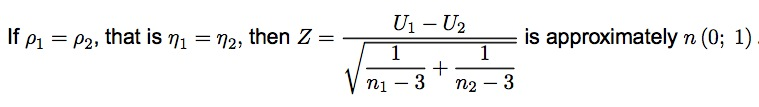
\includegraphics[scale=0.5]{./img/eqcor.jpg}

\h{Study Unit 6}

\sh{Single sample}
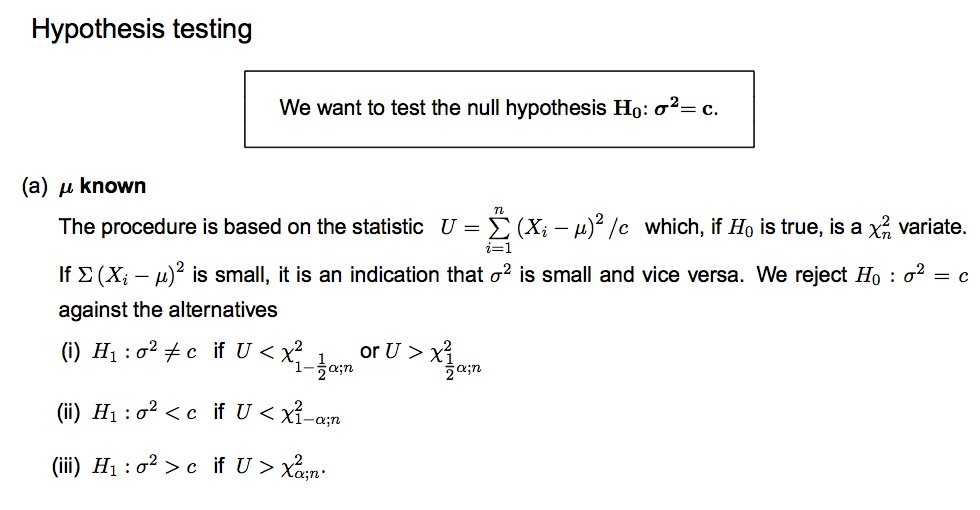
\includegraphics[scale=0.5]{./img/st61.jpg}
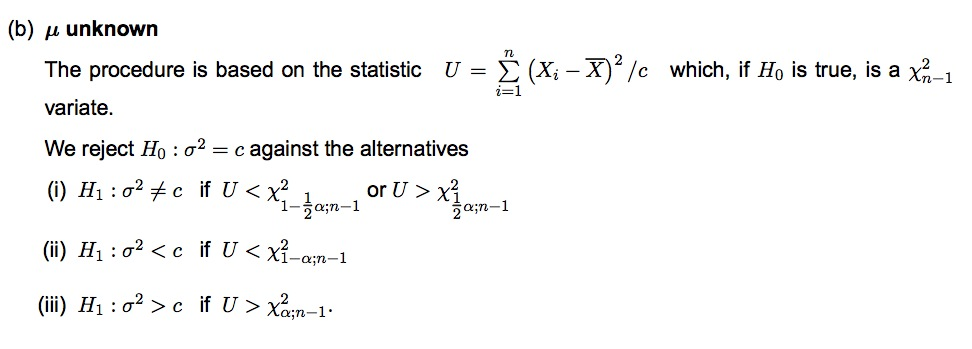
\includegraphics[scale=0.5]{./img/st62.jpg}


\sh{Two independent samples}
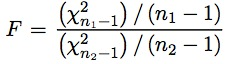
\includegraphics[scale=0.5]{./img/derf.jpg}
yields test statistic
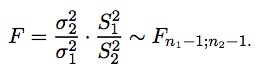
\includegraphics[scale=0.5]{./img/fstat.jpg} 

Hypotheses:
$H_0: \frac{\sigma^2_2}{\sigma^1_2} = c$
$H_1: \frac{\sigma^2_2}{\sigma^1_2} \ne c$
$H_1: \frac{\sigma^2_2}{\sigma^1_2} < c$
$H_1: \frac{\sigma^2_2}{\sigma^1_2} > c$

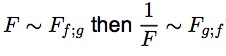
\includegraphics[scale=0.5]{./img/invf.jpg}

\sh{Paired observations}
$H_0: \sigma^2_1=\sigma^2_2$
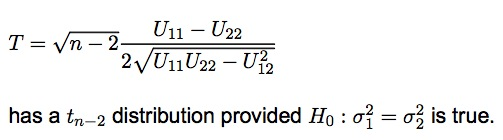
\includegraphics[scale=0.5]{./img/r61.jpg}

$U_{11}=\sum(X_{1j}-\bar{X_1})^2$
$U_{22}=\sum(X_{2j}-\bar{X_2})^2$
$U_{12}=\sum(X_{1j}-\bar{X_1})(X_{2j}-\bar{X_2})$
Multiply out to get calculator formulas.

\sh{More than two independent samples}

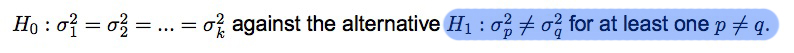
\includegraphics[scale=0.5]{./img/64hyp.jpg}
Test Statistic
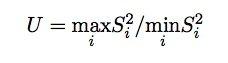
\includegraphics[scale=0.5]{./img/64ts.jpg}
$n-1$ degrees of freedom, $n=$ size of samples.
$k=$ number of sample variances.

\h{Study Unit 7}
\sh{One Sample Problem}
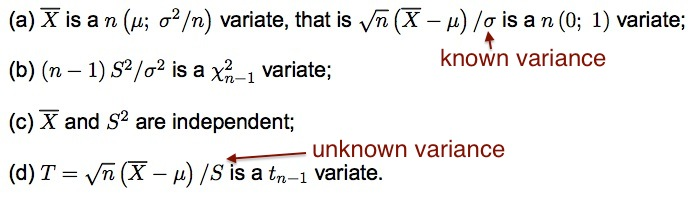
\includegraphics[scale=0.5]{./img/71.jpg}
95\% Tolerance Interval: 95\% confidence that at least 90\% of the population data lie between x and y.

\sh{Power of the test.}
Given that $Z_0$ is standard normal Solve for $\bar{X}$ at significance level.
Then use $\beta$ = P(type II error) =  P($H_0$ is not rejected|$H_1$ is true) 
and standardise using do not reject signs and get probability 
Then power of test is 1-$\beta$

\sh{Two-sample problem, independent samples. same variance}
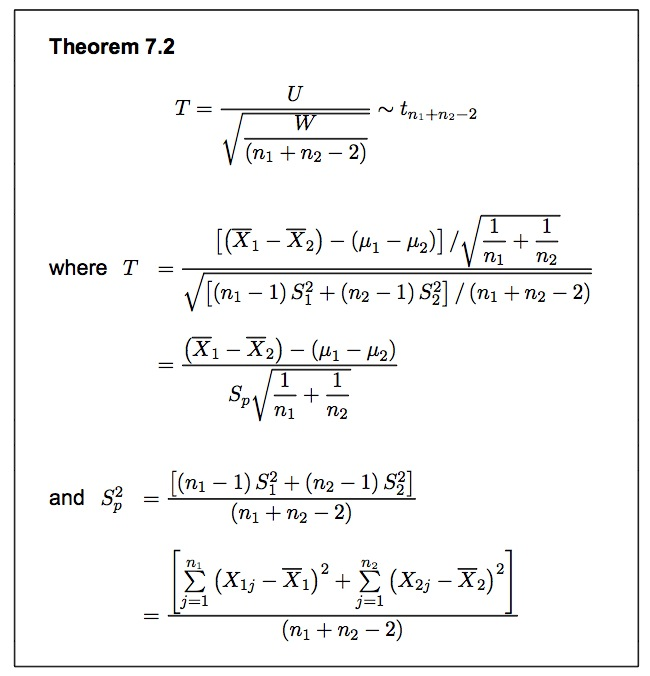
\includegraphics[scale=0.5]{./img/72.jpg}
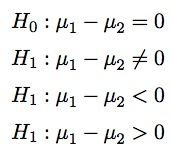
\includegraphics[scale=0.5]{./img/72hyp.jpg}

\sh{Paired observations}
Same as one sample problem, by transforming by subtraction, then use $T=\displaystyle\frac{\sqrt{n}(\bar{Y}-\mu)}{S_Y}$

\sh{Independent samples with unequal variances}
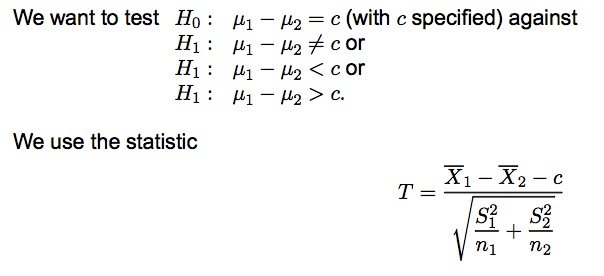
\includegraphics[scale=0.5]{./img/75.jpg}
to get degrees of freedom, use formula and the interpolate table III.
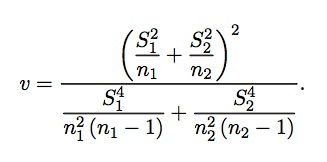
\includegraphics[scale=0.5]{./img/v.jpg}

\sh{More than two independent samples One-way ANOVA}
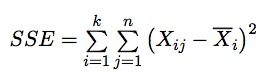
\includegraphics[scale=0.5]{./img/sse.jpg}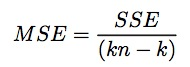
\includegraphics[scale=0.5]{./img/mse.jpg}
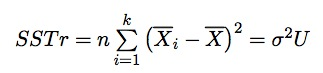
\includegraphics[scale=0.5]{./img/sstr.jpg}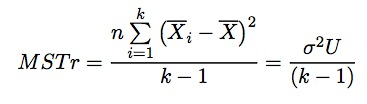
\includegraphics[scale=0.5]{./img/mstr.jpg}
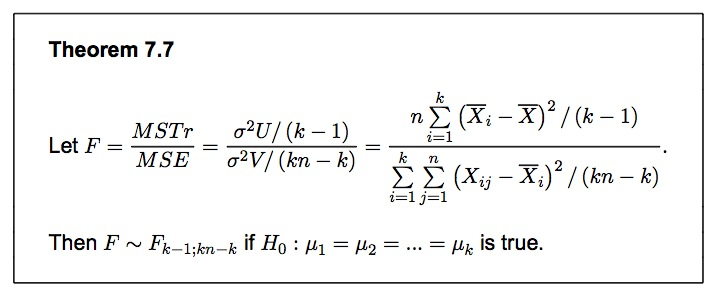
\includegraphics[scale=0.5]{./img/annovaf.jpg}
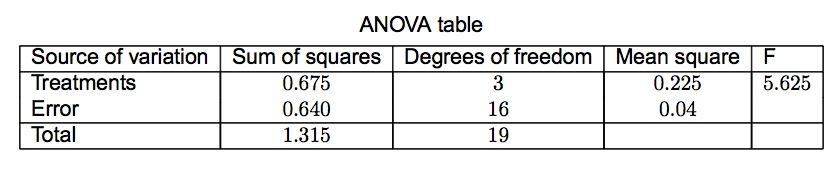
\includegraphics[scale=0.5]{./img/anova.jpg}

\sh{Multiple comparisons for ANOVA}
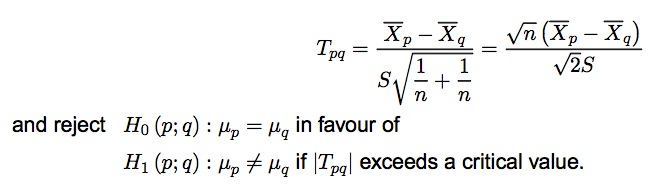
\includegraphics[scale=0.5]{./img/muc.jpg}
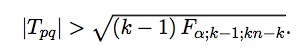
\includegraphics[scale=0.5]{./img/muc2.jpg}

\h{Study Unit 8}
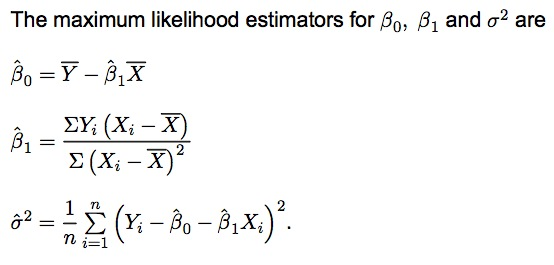
\includegraphics[scale=0.5]{./img/81.jpg}
$\hat{\beta}_1=\displaystyle\frac{\sum(X-r\bar{X})(Y-\bar{Y})}{\sum(X-\bar{X})^2}$

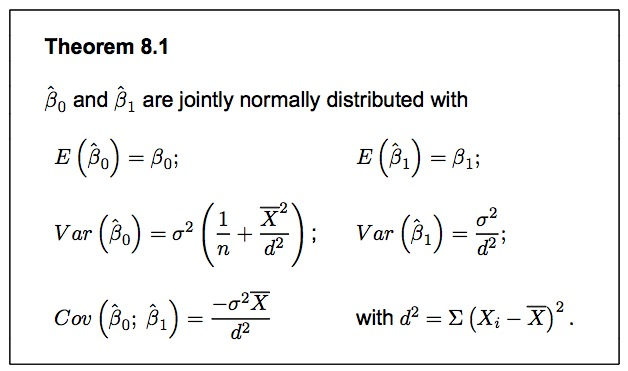
\includegraphics[scale=0.4]{./img/t81.jpg}
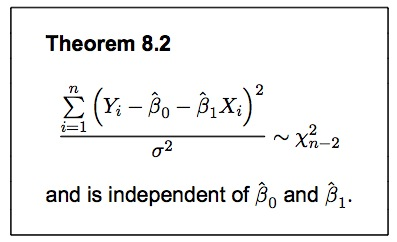
\includegraphics[scale=0.4]{./img/t82.jpg}
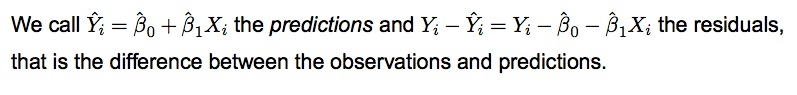
\includegraphics[scale=0.5]{./img/8216.jpg}

\sh{Inference on the coefficients}
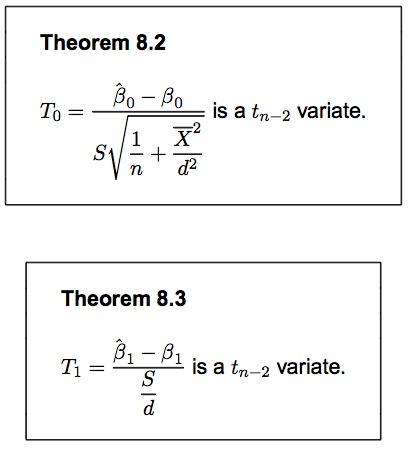
\includegraphics[scale=0.4]{./img/84.jpg}
Variance around regression line:
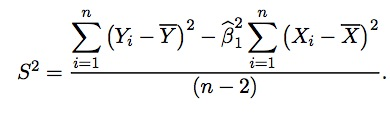
\includegraphics[scale=0.5]{./img/s2.jpg}

Confidence interval for $B_0$
\includegraphics[scale=0.5]{./img/b0c.jpg}
Confidence interval for $B_1$
\includegraphics[scale=0.5]{./img/b1c.jpg}

\sh{Inference on the regression line}


\includegraphics[scale=0.5]{./img/851.jpg}
\includegraphics[scale=0.5]{./img/852.jpg}
\includegraphics[scale=0.5]{./img/853.jpg}

\sh{Relationship between test for correlation and regression}
\includegraphics[scale=0.5]{./img/s21.jpg}
\includegraphics[scale=0.5]{./img/s22.jpg}


$Var(\sum{b_iY_i})=\sigma^2\sum{b^2_i}$

to standardise: $\displaystyle\frac{X-\Epsilon(X)}{\sqrt{\mathrm{Var}(x)}}$



\end{document}
 
